\documentclass[11pt]{beamer}
\usepackage{amsfonts,amsmath,amsthm,amssymb}
\theoremstyle{plain}
\newtheorem{conjecture}{Conjecture}[section]
\usepackage{mathtools,mathptmx,listings,forest,enumitem}
\usepackage{graphicx}
\usepackage{pgfplots}
\pgfplotsset{compat=newest}
% plotting things
\usepackage{graphicx}
\graphicspath{{images/}}
\usepackage{tikz-cd}
\pgfplotsset{compat=1.15}
\usepackage[
	backend=biber,
	style=verbose,
	sorting=ynt
]{biblatex}
\addbibresource{references.bib}
\usetheme{Madrid}
\usepackage{float,mathtools,dirtytalk,ulem,csquotes,cancel,hyperref}
\author[] % (optional)
{Emon Hossain\inst{1}}

\institute[University of Dhaka] % (optional)
{
  \inst{1}%
  Lecturer\\MNS department\\Brac University
}

\date[] % (optional)
{\textsc{Lecture-02}}


\title[]{MAT215: Complex Variables And Laplace Transformations}

\setbeamertemplate{navigation symbols}{}


\AtBeginSection[]
{
  \begin{frame}
    \frametitle{Table of Contents}
    \tableofcontents[currentsection]
  \end{frame}
}

\usepackage{Kyushu}

% \usetheme{Frankfurt}

\begin{document}
\begin{frame}
\titlepage
\end{frame}

\begin{frame}{Parametrization}
    The key to parametrization is to realize that the goal of this method is to describe the location of all points on a geometric object, such as a curve, a surface, or a region. This description must be one-to-one and onto: every point must be described once and only once.
    $$\gamma:=\{(x,y): x^2+y^2=1\}$$
If you want to geometrically analyze the curve $\gamma$ (length/enclosed area, etc), we need a manageable way to produce the points (production scheme). 
\end{frame}

\begin{frame}{Motivation of Parametrization}
    Parametric curve: A curve in the 2-D plane can be described by,
$$
\left.\begin{array}{l}
x=f(t) \\
y=g(t)
\end{array}\right\} \text { where } a \leqslant t \leqslant b
$$
These are called parametric equations for that curve, and $t$ is the parameter. 
$$\boxed{\text{What is the difference between general and parametric curves?}}$$
\end{frame}

\begin{frame}{Example}
Plot the parametric curves defined by,
\begin{itemize}
    \item $x=\cos t, y=-\sin t ; 0 \leq t \leq \pi$
    \item $x=t, y=1 ; 0 \leq t \leq 4$
    \item $z=1+i t ; 0 \leq t \leq 1$ 
    \item Straight line from $(0,3)$ to $(2,3)$
    \item Straight line from $(2,3)$ to $(2,4)$
    \item Straight line from $(0,3)$ to $(2,4)$
\end{itemize}
\end{frame}

\begin{frame}{Formula}
    $$\boxed{\text{Line segment: }\gamma(t)= a+t(b-a), 0\leq t\leq 1}$$
    $$\boxed{\text{Circle: }\gamma(t)=(a+r\cos(t),b+r\sin(t)) , 0\leq t\leq 2\pi}$$
    $$\boxed{\text{Explicit function: }\gamma(t)\stackrel{y=f(x)}{=}(t,f(t))}$$
    $$\boxed{\text{Explicit function in polar: }\gamma(t)\stackrel{r=f(\theta)}{=}(f(t)\cos(t),f(t)\sin(t))}$$
\end{frame}

\begin{frame}{Smooth Curves}
    Derivative exists at all points and is continuous 
\end{frame}

\begin{frame}{Motivation of line integral}
\begin{figure}
    \centering
    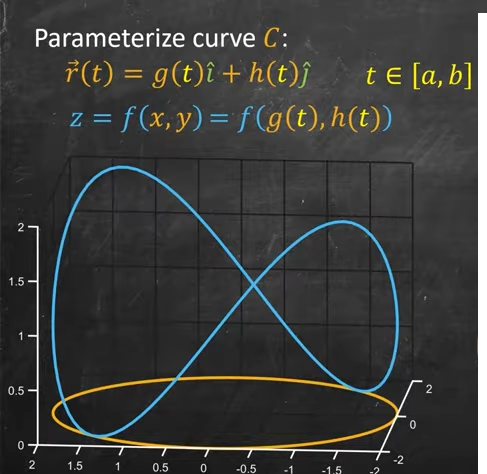
\includegraphics[width=0.5\linewidth]{Line_integral.png}
\end{figure}
\end{frame}

\begin{frame}{continued...}
    \begin{figure}
        \centering
        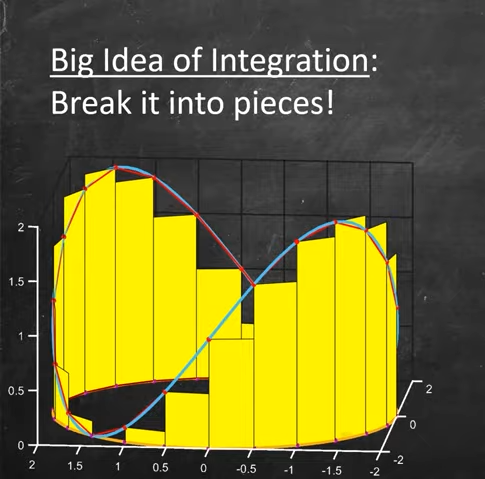
\includegraphics[width=0.5\linewidth]{line_integral_2.png}
    \end{figure}
\end{frame}

\begin{frame}{Path in complex integration}
    Is there any meaning of $$\int_{z_1}^{z_2}f(z)dz=?$$
    \pause
    Consider $C:z(t)=h(t)+ig(t); a\leq t\leq b$
    Then line integral (or complex line integration) of $f$ along $C$ is defined as, 
    $$\int_C f(z) dz=\int_a^b f(\gamma(t))\gamma'(t)dt$$
\end{frame}


\begin{frame}{Example}
    $C_1:z(t):=\gamma(t)=t, 0\leq t\leq 1$\\
    $C_2:z(t)=1+it, 0\leq t\leq 1$\\
    $f(z)=\bar z$
    $C_3:z(t)=\gamma(t)=t(1+i),0\leq t\leq 1$
\end{frame}

\end{document}